
\begin{figure}
    \centering
    
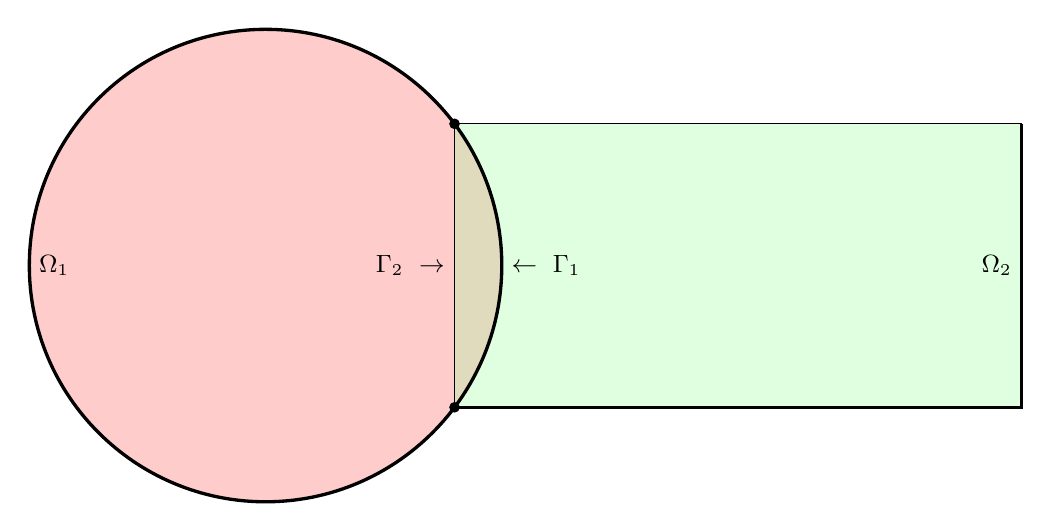
\begin{tikzpicture}[scale=0.6]%[transform canvas={scale=0.6}]
    \filldraw[fill=red,draw=black,fill opacity = 0.2](0,0) circle (5);
    \filldraw[fill=green!40!white, draw=black,fill opacity=0.3] (4,-3) rectangle (16,3);
    %\draw [white,very thin] (4,-3) -- (4,3);
    \draw[very thick] (0,0) circle (5);
    \draw[very thick] (4,-3) -- (16,-3) -- (16,3) ;
    \filldraw[fill=black](4,3) circle [radius = 0.1];
    \filldraw[fill=black](4,-3) circle [radius = 0.1];
    \draw (-5,0) node[anchor=west]{\fontsize{9bp}{10pt}\selectfont $\Omega_1$};
    \draw (4,0) node[anchor=east]{\fontsize{9bp}{10pt}\selectfont $\Gamma_2\  \rightarrow$};
    \draw (5,0) node[anchor=west]{\fontsize{9bp}{10pt}\selectfont $\leftarrow\  \Gamma_1$};
    \draw (16,0) node[anchor=east]{\fontsize{9bp}{10pt}\selectfont $\Omega_2$};
\end{tikzpicture}
\caption{\fontsize{9bp}{18bp}\selectfont Schwarz交替法示意图} \label{fig:schwarzalter}
\end{figure}
